\documentclass[12pt,a4paper]{article}

\usepackage[T1,T2A]{fontenc}
\usepackage[utf8]{inputenc}
\usepackage[english, russian]{babel}
\usepackage{indentfirst}
\usepackage{misccorr}
\usepackage{graphicx}
\usepackage{amsmath}
\usepackage{graphicx}
\usepackage{float}
\usepackage[left=20mm,right=10mm, top=20mm,bottom=20mm,bindingoffset=0mm]{geometry}

\setlength{\parskip}{6pt}
\DeclareGraphicsExtensions{.png}

\begin{document}

    \begin{titlepage}
        \begin{center}
            \large
            Санкт-Петербургский политехнический университет\\Петра Великого\\
            \vspace{0.5cm}
            Институт прикладной математики и механики\\
            \vspace{0.25cm}
            Кафедра «Прикладная математика»
            \vfill
            \textsc{\LARGE\textbf{Отчет по лабораторной работе №3}}\\[5mm]
            \Large
            по дисциплине\\"Математическая статистика"
        \end{center}
        \vfill
        \begin{tabular}{l p{175} l}
            Выполнила студентка\\группы 3630102/80201 && Деркаченко Анна Олеговна
            \vspace{0.25cm}
            \\Проверил\\доцент, к.ф.-м.н. && Баженов Александр Николаевич
        \end{tabular}
        \vfill
        \begin{center}
            Санкт-Петербург\\2021 г.
        \end{center}
    \end{titlepage}

\newpage
\begin{center}
    \tableofcontents
    \setcounter{page}{2}
\end{center}
\newpage
\begin{center}
    \listoffigures
\end{center}

\newpage
\section{Постановка задачи}
Даны распределения:
\begin{itemize}
    \item нормальное распределение $N(x,0,1)$
    \item распределение Коши $C(x,0,1)$
    \item распределение Лапласа $L(x,0,\frac{1}{\sqrt{2}})$
    \item распределение Пуассона $P(k,10)$
    \item равномерное распределение $U(x,-\sqrt{3},\sqrt{3})$
\end{itemize}

Необходимо:
\begin{enumerate}
    \item Сгенерировать выборки размером 20 и 100 элементов
    \item Построить для них боксплот Тьюки
    \item Для каждого распределения определить долю выбросов экспериментально (сгенерировав выборку, соответствующую распределению 1000 раз, и вычислив среднюю долю выбросов) и сравнить с результатами, полученными теоретически
\end{enumerate}

\section{Теория}
\subsection{Боксплот Тьюки}
\textit{Боксплот Тьюки} - график, использующийся в описательной статистике, компактно изображающий одномерное распределение вероятностей. Данный вид диаграммы в удобной форме показывает множество характеристик положения случайной величины.

Построение боксплота производится по следующим параметрам:
\begin{itemize}
    \item границы боксплота - $Q_1$, $Q_3$ - первый и третий квартили соответственно
    \item линия середины боксплота - медиана
    \item концы "усов" - края статистически значимой выборки (без выбросов). Их длина определяется по формуле:
        \begin{equation}
            X_1=Q_1-\frac{3}{2}(Q_3-Q_1)
            X_2=Q_3+\frac{3}{2}(Q_3-Q_1)
        \label{eq:mustache}
        \end{equation}
        , где $X_1$ — нижняя граница уса, $X_2$ — верхняя граница уса
    \item выбросы - данные, выходящие за границы усов, отображающиеся на графике в виде кружков
\end{itemize}

\subsection{Теоретическая вероятность выбросов}
После вычисления первого и третьего квартилей и нижней и верхней границы уса по формуле \eqref{eq:mustache}, можно определить выбросы $x:$
\begin{equation}
	\left[
	\begin{array}{ll}
        x<X_1^T\\
		x>X_2^T\\
	\end{array}
    \right.
\end{equation}

Пусть $F(X)=P(x\leq{X})$ - функция распределения. Теоретическая вероятность выбросов
\begin{itemize}
    \item для непрерывных распределений:
        \begin{equation}
		    P_B^T=P(x<X_1^T)+P(x>X_2^T)=F(X_1^T)+(1-F(X_2^T))
	    \end{equation}
	\item для дискретных распределений:
	    \begin{equation}
		    P_B^T=P(x<X_1^T)+P(x>x_2^T)=(F(X_1^T)-P(x=X_1^T))+(1-F(X_2^T))
	    \end{equation}
\end{itemize}

\section{Реализация}
Реализация лабораторной работы проводилась на языке Python в среде разработки PyCharm c использованием дополнительных библиотек:
\begin{itemize}
    \item scipy
    \item numpy
    \item math
    \item matplotlib
    \item seaborn
\end{itemize}

Исходный код лабораторной работы размещен в GitHub-репозитории.

URL: https://github.com/derkanw/Mathstat/tree/main/lab3

\section {Результаты}
\subsection{Боксплот Тьюки}
\begin{figure}[H]
    \centering
    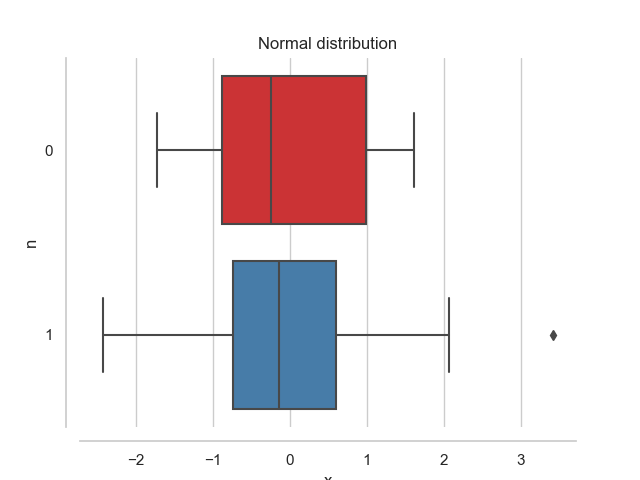
\includegraphics[scale=0.8]{images/normal.png}
    \caption{Нормальное распределение}
    \label{fig:normal}
\end{figure}

\begin{figure}[H]
    \centering
    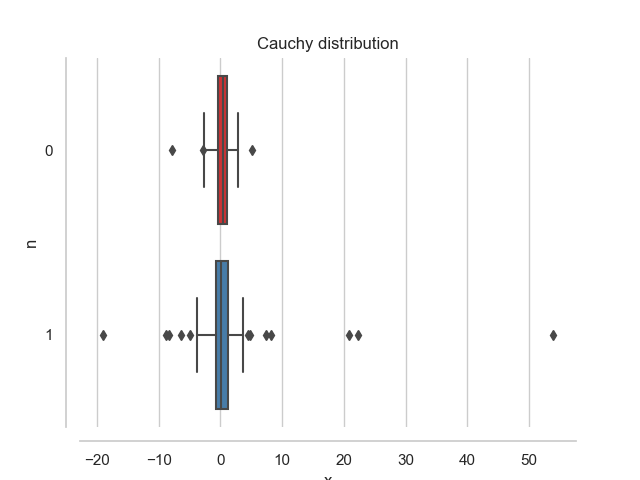
\includegraphics[scale=0.8]{images/cauchy.png}
    \caption{Распределение Коши}
    \label{fig:cauchy}
\end{figure}

\begin{figure}[H]
    \centering
    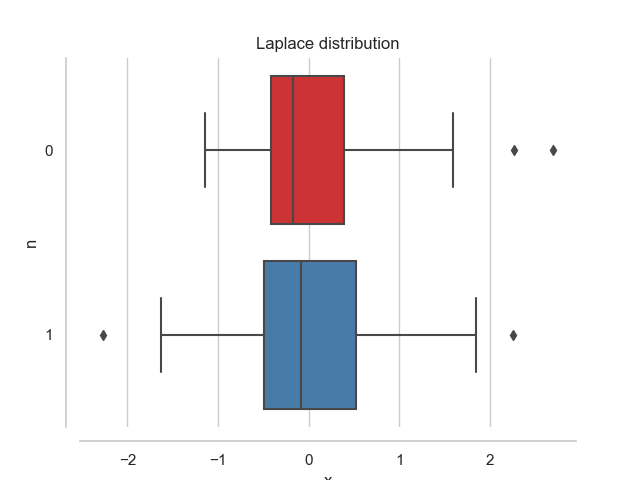
\includegraphics[scale=0.8]{images/laplace.png}
    \caption{Распределение Лапласа}
    \label{fig:laplace}
\end{figure}

\begin{figure}[H]
    \centering
    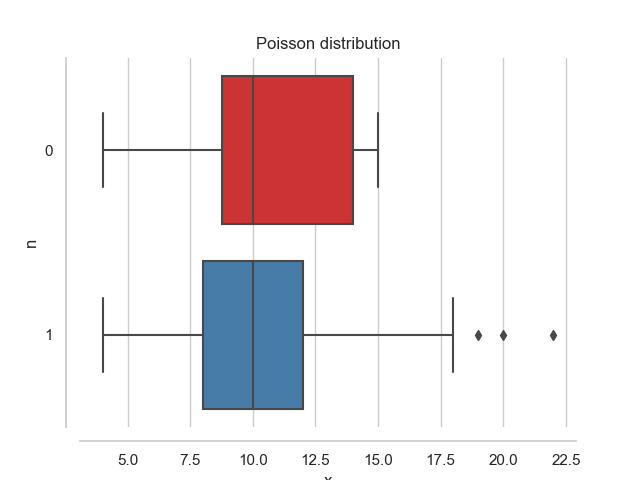
\includegraphics[scale=0.8]{images/poisson.png}
    \caption{Распределение Пуассона}
    \label{fig:poisson}
\end{figure}

\begin{figure}[H]
    \centering
    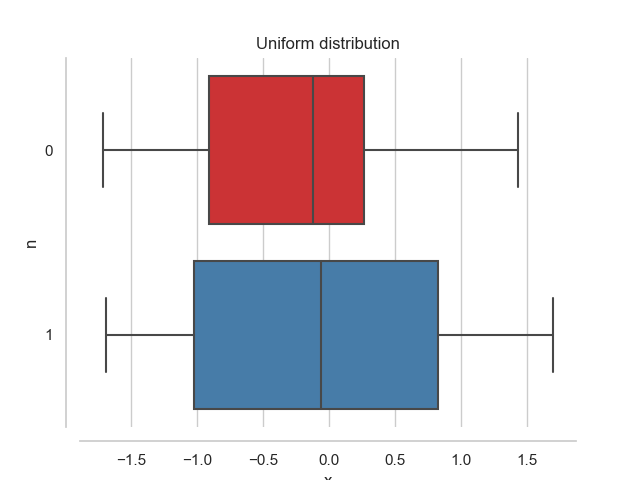
\includegraphics[scale=0.8]{images/uniform.png}
    \caption{Равномерное распределение}
    \label{fig:uniform}
\end{figure}

\subsection{Доля выбросов}
\begin{table}[H]
	\centering
	\begin{tabular}{|l|c|c|}
		\hline
		Выборка & Доля выбросов	& $P^T_B$\\\hline
		\hline
		Normal n = 20 & 0.02285 & 0.007\\\hline
		Normal n = 100 & 0.00959 & 0.007\\\hline
		Cauchy n = 20 & 0.1526 & 0.156\\\hline
		Cauchy n = 100 & 0.15549 & 0.156\\\hline
		Laplace n = 20 & 0.0744 & 0.063\\\hline
		Laplace n = 100 & 0.06626 & 0.063\\\hline
		Poisson n = 20 & 0.02375 & 0.008\\\hline
		Poisson n = 100 & 0.00956 & 0.008\\\hline
		Uniform n = 20 & 0.00265 & 0\\\hline
		Uniform n = 100 & 0 & 0\\\hline
	\end{tabular}
	\caption{Практическая доля выбросов}
\end{table}

\begin{table}[H]
	\centering
	\begin{tabular}{|l|c|c|c|c|c|}
		\hline
		Распределение & $Q_1^T$	& $Q_3^T$ & $X_1^T$ & $X_2^T$ & $P_B^T$\\\hline
		\hline
		Нормальное & -0.674 & 0.674 & -2.698 &  2.698 & 0.007\\\hline
		Коши & -1 & 1 & -4 & 4 & 0.156\\\hline
		Лапласа & -0.490 & 0.490 & -1.961 & 1.961 & 0.063\\\hline
		Пуассона & 8 & 12 & 2 & 18 & 0.008\\\hline
		Равномерное & -0.866 & 0.866 & -3.464 & 3.464 & 0\\\hline
	\end{tabular}
	\caption{Теоретическая вероятность выбросов}
\end{table}

\section{Обсуждение}
Боксплот Тьюки позволяет наглядно представить характеристики заданного распределения, такие как медиана, первый и третий квартили, наличие выбросов. К тому же процесс анализа данной диаграммы удобнее, нежели полный аналитический расчет.

Судя по данным таблиц для различных выборок, в большинстве случаев наблюдается закономерность: чем больше размерность выборки, тем ближе найденная доля выбросов к теоретической оценке. Практическая и теоретическая доля выбросов для распределения Коши имеют значения, значительно превышающие аналогичные для остальных распределений, что говорит о относительно частом возникновении выбросов при использовании данного распределения. Стоит сказать, что у равномерного распределения, наоборот, выбросы почти не наблюдаются.
\end{document}
